\cchapter{مروری بر ادبیات}
\label{literature}
در این بخش سعی داریم تا با مروری بر اصطلاحات و ابزارهای مورد استفاده در پژوهش‌های بررسی شده، با پیش‌نیازهای مبحث موردنظر آشنا شویم. 
\section{رایانش بدون سرور}
رایانش بدون سرور\LTRfootnote{Serverless Computing} در سال 2014 توسط شرکت آمازون برای اولین بار معرفی شد. تا قبل از این رایانش بدون سرور یک مفهوم انتزاعی \LTRfootnote{abstract} در شبکه بود که شرکت آمازون با ارائه پلتفرم \lr{AWS Lambda Functions} \cite{aws} به معرفی آن پرداخت. سپس در سال 2016 سایر ارائه دهندگان خدمات ابری نیز به ارائه پلتفرم‌های بدون سرور خود پرداختند. در این سال به ترتیب شرکت‌های گوگل پلتفرم \lr{google cloud functions} یا به اختصار \lr{GCP}، شرکت مایکروسافت پلتفرم \lr{Microsoft Azure functions} و شرکت \lr{IBM} به معرفی \lr{IBM OpenWhisk} پرداختند. البته باید توجه داشت که مفهوم رایانش بدون سرور به طور کامل توسط ارائه دهندگاه خدمات ابری پیاده‌سازی نشده است و جای کار بسیاری دارد (با مطالعه این گزارش به مرور متوجه نواقص موجود خواهید شد).

در رایانش بدون سرور ما از نقطه قوت ماشین‌های مجازی که ایزولاسیون برنامه‌های مختلف از همدیگر بود استفاده کرده‌ایم. منتها این مورد را با مفهوم کانتینر ها پیاده‌کرده ایم. در ادامه راجع به کانتینرها نیز بحث خواهیم کرد. 

\subsection{تعریف رایانش بدون سرور}
\par
رایانش بدون سرور مبحثی از رایانش ابری است که در آن بحث مدیریت حافظه یا \lr{Storage}، مدیریت زیرساخت و بحث‌های \lr{networking} با انتزاع بالایی به مصرف کاربر می‌رسد. به عبارت دیگر، تمامی مدیریت ای بخش‌ها بر عهده ارائه دهندگان است و ما اصلا با این بحث ها سروکاری نداریم. در واقع، هدف اصلی رایانش بدون سرور هم این است که این پیچیدگی‌ها را از کاربر بگیرد. 

\par
به طور کلی، یک‌ پلتفرم بدون‌سرور را هر پلتفرم محاسباتی تعریف کرد که در آن مدیریت مستقیم سرور از کاربران مخفی شده و برنامه‌های کاربردی به صورت اتوماتیک در آن مقیاس‌پذیر می‌شوند و تنها هنگامی که در حال استفاده از پلتفرم هستیم، هزینه آن را پرداخت می‌کنیم. \cite{The_Rise_of_Serverless_Computing}

\par
بسیاری از افراد، \lr{serverless} و \lr{faas} را معادل یک‌دیگر می‌دانند درحالی‌که اصلا این‌گونه نیست. در ادامه راجع به این بحث به طور مفصلی بحث خواهیم کرد اما باید بدانیم که این دو مقوله کاملا جدا از همدگیر هستند و مجددا تاکید می‌کنیم که رایانش بدون سرور یک مدل اجرایی در رایانش ابری است. 

\par
ازطرفی رایانش بدون سرور را باید نقطه مقابل رایانش سرور آگاهانه \LTRfootnote{Server Aware} دانست که در آن از اطلاعات سرور در اختیار گرفته کاملا اگاهیم، کاملا بر مدیریت آن اشراف داریم و هرگونه تغییر از جمله متعادل‌سازی بارها، \lr{auto-scaling} و … باید توسط کاربر انجام شود.

\par
یک مثال از پیاده‌سازی رایانش سرور آگاهانه را در زیرساخت به عنوان سرویس \LTRfootnote{Infrastructure as a service} یا به اختصار \lr{IaaS} است. در نقطه مقابل در رایانش بدون سرور هیچ کنترلی بر روی سرور نداریم، تنها می‌توانیم یک برنامه را بر روی سرور اجرا کنیم یا اجرای آن را به حالت تعلیق درآورده یا آن را از روی سرور حذف کنیم که هیچ‌کدما از این موارد نیز به صورت مستقیم انجام نمی‌گیرد؛ بلکه رابط گرافیکی و \lr{API} وجود دارد که از طریق آن‌‌ها این تغییرات را اعمال می‌کنیم. بنابراین در رایانش بدون سرور، عملا هیچ راهی برای مدیریت مستقیم سرور و زیرساخت نداریم.

شکل \ref{fig:ServerlessVSServeraware} مرز‌های بین رایانش بدون‌سرور و رایانش سرور آگاهانه را نمایش می‌دهد.  

\begin{figure}
	\centering
	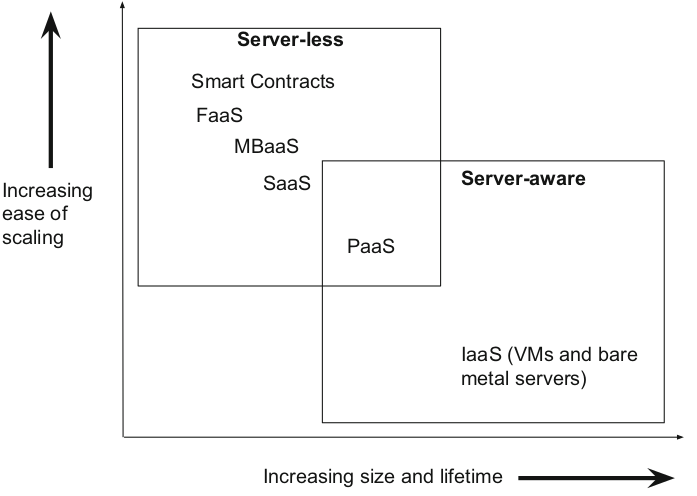
\includegraphics[width=\linewidth]{figs/ServerlessVSServeraware}
	\caption {مرز‌های رایانش بدون سرور و رایانش سرورآگاهانه}
	\label{fig:ServerlessVSServeraware}
\end{figure}

\par
البته باید به این نکته توجه‌داشت که امروزه مرز‌های بین رایانش سرور آگاهانه با رایانش بدون سرور در حال کمرنگ شدن و بعضا از بین رفتن است و این تقسیم بندی ابدا قاطعیت ندارد.همچنین تفکیک برخی موارد مانند \lr{Platform-as-a-Serice} یا به اختصار \lr{PaaS} به راحتی انجام نمی‌گیرد بلکه این نوع رایانش می‌تواند از نوع باسرور یا بدون سرور باشد. 
در این شکل هرچه به سمت محور افقی حرکت می‌کنیم دانه‌بندی و طول‌عمر افزایش پیدا می‌کند و هرچه به سمت بالاتر می‌رویم، \lr{scalingz} راحت‌تر انجام می‌گیرد. 

\par
از مزایای رایانش بدون سرور همچنین می‌توان به پشتیبانی و توسعه راحت‌تر اپلیکیشن‌ها با معماری میکروسرویس و نانوسرویس هم اشاره کرد. البته معماری نانوسرویس مبحث جدیدتری است و جای پژوهش‌های بیشتری دارد.

\subsection{معماری}
\par
واژه serverless ممکن است این تفکر را به ذهن مبتدر سازد که اصلا در این نوع مدل رایانشی سروری نداریم؛ در حالی‌که این امر بسیار اشتباه است. در رایانش بدون سرور اگرچه سروری برای مدیریت به کاربر اختصاص داده نمی‌شود اما این موضوع بدان معنا نیست که اصلا سروری در کار نیست. در واقع مانند تمامی مدل‌های رایانشی در این‌جا هم سرور داریم، ولی تمامی تصمیمات مثل توزیع بار، تعداد اپ‌های روی سرور، انتخاب سرور‌ها برای اجرای اپلیکیشن، کانفیگ CI/CD و … بر عهده ارائه دهنده خدمات ابری است. اما برای درک نحوه کار یک پلتفرم بدون سرور، بهتر است با معماری آن آشنا باشیم. شکل \ref{fig:Serverless-Architecture} معماری یک پلتفرم خدمات ابری را نشان می‌دهد.

\par

\begin{figure}
	\centering
	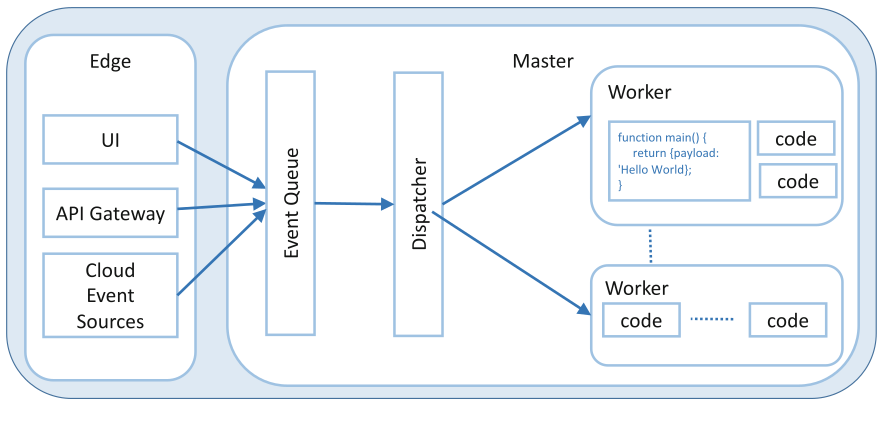
\includegraphics[width=\linewidth]{figs/Serverless-Architecture}
	\caption {معماری کلی یک پلتفرم بدون سرور}\LTRfootnote{Serverless Platform Architecture}
	\label{fig:Serverless-Architecture}
\end{figure}

\par
همانگونه که در تصویر مشخص است دوبخش کلی داریم، بخش لبه\LTRfootnote{edge}‌ و بخش رییس \LTRfootnote{master}، بخش لبه شامل رابط گرافیکی کاربر\LTRfootnote{User Interface}، API Gateway و \lr{Cloud Event Source} می‌شود که برای تعامل با سرور رییس\LTRfootnote{master server} مناسب هستند. از طرف دیگر، در سرور رییس، درخواست‌ها ابتدا به صف رخداد‌ها\LTRfootnote{Event Queue} رسیده. صف رخداد‌ها مسئول مدیریت رخداد و نظم‌دهی به آن‌ّ‌ها است. هر داده در صف رخ‌داد نوبت‌دهی می‌شود و سپس به بخش توزیع‌کننده\LTRfootnote{dispatcher} می‌رود. توزیع‌کنند آپلیکیشن را برای دیپلوی، یا درخواست را برای سرویس‌دهی به یک نود کارگر\LTRfootnote{worker node} هدایت می‌کند نود کارگر نیز با ارسال کدهای پاسخ\LTRfootnote{Response Code} با سرور رییس در ارتباط است. \cite{baldini2017serverless}

البته بهتر است بدانیم که امروزه ادبیات رییس-کارگر\LTRfootnote{Master-worker} برای نامیدن این معماری منسوخ شده و به جای آن از ادبیات رییس--گره\LTRfootnote{Master-Node} استفاده می‌کنند. 

\subsection{ویژگی‌های پلتفرم‌های بدون سرور}
امروزه پلتفرم‌‌های بدون سرور بسیاری وجود دارند که روزانه بر تعداد آن‌ها افزوده می‌شود. اما باید دنبال ویژگی‌هایی برای آن‌ها باشیم که براساس آن‌ها بتوان این پلتفرم‌ها را تفکیک کرد و دست به مقایسه‌ی آن‌ها زد. 

شاخص‌هایی که در این قسمت بررسی می‌کنیم شاخص‌های کمی و کیفی برای مقایسه‌ی بین این پلتفرم‌ها است. 

\begin{enumerate}
	\item هزینه:
	
	به طور معمول در رایانش بدون سرور، از مدل پرداخت پرداخت-به-ازای-استفاده\LTRfootnote{pay-as-you-go} استفاده می‌کنیم. یک ویژگی اساسی در تمایز بین ارائه‌دهندگان مختلف خدمات ابری، تفاوت آن‌ها در پشتیبانی از ویژگی \lr{scale-to-zero} در این مدل محاسباتی\LTRfootnote{Computational Model} است. این مورد باعث تفاوت معنی‌داری از هزینه‌ها در استفاده از پلتفرم‌‌های مختلف می‌شود. برخی از پلتفرم‌ها هم متن‌باز\LTRfootnote{Open Source} هستند که در این صورت، می‌توان به آسانی آن‌ها را بر روی ماشین مجازی یا سرور شخصی خود پیاده سازی کرد و برای استفاده از خدمات آن متحمل هیچ‌گونه هزینه‌ای نشد.
	
	\item کارایی و محدودیت‌ها\LTRfootnote{Performance and Limits}
	
	 ارائه دهندگان مختلف، محدودیت‌های مختلفی را هم بر روی پلتفرم‌های مختلف خودشان اعمال می‌کنند. این محدودیت‌ها می‌توانند تعداد همزمان درخواست ها (number of concurrent requests)، حداکثر استفاده از RAM و CPU د توسط یک تابع، حداکثر زمان زنده‌ماندن بعد از اجرا توسط تابع و … است. البته برخی از محدودیت‌ها را می‌توان با صرف هزینه یا خرید پلن‌های درامدی سطح بالاتر برطرف کرد. مثلا پلتفرم AWS Lambda functions می‌تواند با صرف هزینه‌ی بیشتری حداکثر تعداد درخواست را افزایش داد. درحالی‌که این مورد در پلتفرم‌های اوپن سورس وجود ندارد. در حالت کلی پلتفرم‌های متن بازی مثل openfaas محدودیت‌های بیشتری را برای کاربر اعمال می‌کنند. علت این امر می‌تواند این باشد که این پلتفرم‌ّها از نظر تکنولوژی و بازدهی (performance) کاملا از همتایان تجاری خود عقب هستند. 
	
	 \item زبان برنامه‌نویسی\LTRfootnote{Programming Languages}
	 
	 پلتفرم‌های بدون سرور از گستره‌ی عظیمی از زبان‌های برنامه‌نویسی پشتیبانی می‌کنند که شامل جاوااسکریپت، گو، پایتون، جاوا، سی‌شارپ، سویفت و پی‌اچ‌پی می‌شود. اکثر پلتفرم‌ها حداقل از ۵ زبان برنامه‌نویسی پشتیبانی می‌کنند. همچنین بسیاری از پلتفرم‌ها مستقل از زبان\LTRfootnote{Language Independent} هستند. یعنی درحالی‌که در داخل کانتینر‌ اجرا می‌شوند (مثلا کانتینر‌های داکر)، دیگر زبان برنامه‌نویسی برای آن‌ها اهمیتی ندارد. این پلتفرم‌ها توابع را در داخل کانتینر اجرا می‌کنند و نتیجه را برمی‌گردانند. 
	 
	 \par
	 \item مدل برنامه‌نویسی \LTRfootnote{Programming Model}
	 
	 مدل‌های مختلفی برای تولید یک متد در پلتفرم‌های بدون سرور داریم. شیوه متداول استفاده از یک متد به نام \lr{main} است که درون آن تابع اصلی تعریف می‌شود. همچنین معمولا ورودی‌های تابع در قالب شیئ‌های \lr{json} تعریف می‌شوند. 
	 
	 \par
	 \item ترکیب توابع\LTRfootnote{Compositions}
	 
	 روش‌های گوناگونی برای اینکه یک تابع‌ یا جریان کاری پیچیده‌را پیاده سازی کنیم وجود دارد. یک روش استفاده از ترکیب‌های توابع است.  تا به حال ۷ ترکیب مختلف شناسایی شده است. پلتفرم‌های تجاری \LTRfootnote{orchestrator}هایی برای پیاده سازی این ترکیبات در خود تعبیه کرده‌آند. متاسفانه پلتفرم‌های متن باز مثل \LTRfootnote{openfaas} از این ترکیب پشتیبانی نمی‌کنند. در ادامه و در بخش کار‌های مرتبط این ویژگی‌ها مطرح خواهند شد.  کاربرد اصلی ترکیب توابع پیاده‌سازی عملکرد‌های پیچیده در پلتفرم‌ بدون سرور است.
	 
	 \par
	 \item استقرار\LTRfootnote{Deployments}
	 
	 پلتفرم‌ها سعی می‌کنند پیاده‌سازی‌ها در رایانش بدون سرور را تا حد ممکن ساده کنند. این یکی از دلایل به وجود آمدن این مدل رایانشی بوده. به صورت معمول پلتفرم‌ها برنامه‌ها را در قالب کانتینر‌های داکری دریافت می‌کنند و درون کانتینر مربوطه کد را اجرا می‌کنند. علاوه بر داکر پلن‌هایی از جمله دریافت کد باینری، دریافت سورس کد و سپس کانینرایز کردن آن وجود دارد.
	 
	 \item امنیت و حسابدری\LTRfootnote{Security and Accounting}
	 
	 این دو مورد در کنارهمدیگر به کار برده می‌شوند که معمولاخارج از بحث‌های رایانش ابری کاملا جدا از همدیگر به کار برده می‌شوند. در رایانش بدون سرور لازم است که اپ‌ها کاملا از همدگیر جدا اجرا شوند به این دلیل که بتوانیم برای هر کاربر هزینه‌ای که باید پرداخت کند را محاسبه کنیم. درصورتی که اجرای کاربران از همدگیر تفکیک شده نباشد، محاسبه‌ی هزینه ممکن نیست. اما اجرای جداگانه‌ی توابع از یکدیگر علت دیگری نیز دارد، امنیت. لازم است که توابع جداگانه اجرا شوند تا در توابع و کاربران نتوانند در کار‌های همدیگر دخالتی داشته باشند. این مورد حتی می‌تواند باعث به وجود آمد باگ‌های امینتی و دسترسی کاربران به سیستم کاربران دیگر از طریق مدل رایانشی ما شود.
	 
	 \item پایش و اشکال زدایی\LTRfootnote{Monitoring and Debugging}
	 
	 هر پلتفرم رایانشی امکاناتی از جمله پایش اولیه برای درخواست‌ها را به کاربر می‌دهد. البته این بحث یکی از مسائل باز در این حوزه است و نیاز به بررسی بیشتری دارد. در حال حاضر دیباگینگ از طریق تجزیه و تحلیل لاگ‌های سیستم ممکن است ولی ممکن است در آینده بهبود‌هایی در این حوزه حاصل شود. علت اینکه دیباگینگ بسیار چالش برانگیز است این است که در رایانش بدون سرور اپ‌های ما کانتینرایز می‌شوند و چون محیط کانتیر محیطی ایزوله است، امکان مطالعه و دیباگینگ ممکن نیست. بعلاوه توابع تنها در حالت استفاده در پلتفرم زنده هستند؛ پس مدت زمان اشکال‌زدایی ما نیز بسیار محدود می‌شود. باید به این نکته دقت داشت که به طور متوسط در رایانش بدون سرور، توابع 99درصد زمان را از تاریخ استقرار روی سرور، درخواب هستند.
	 اما در مورد پایش نرم‌افزار پلتفرم بدون سرور در داشبورد مدیریتی خود امکاناتی جهت مشاهده منابع مصرف شده، منابع آزاد مدت زمان استفادهشده، تعداد درخواست‌ها و فراخوانی ها، تعداد شروع‌های سرد و … دارد. به‌علاوه ابزارهای پایش مانند      \lr{prometheus} به خوبی با این پلتفرم‌ها امکان اتصال دارند و با پنل‌هایی مانند \lr{grafana} می‌توان از مانیتورینگ مضاعف برای این سرور‌ها بهره برد.
\end{enumerate}

\subsection{پلتفرم‌های تجاری}

پلتفرم‌های اندکی برای این قسمت وجود دارد. معروف‌ترین آ‌ن‌ها عبارتند از : \lr{AWS Lambda Funcitons} ، \lr{Google Cloud Functions}، \lr{Microsoft Azure Functions} و \lr{IBM OpenWhisk}

\begin{enumerate}
	\item \lr{AWS Lambda Functions}
	
پلتفرم \lr{AWS} \cite{AWSLambda} پلتفرم ارائه شده در بحث رایانش بدون سرور بود که دارای خلاقیت‌های بسیاری بود. از مدل‌برنامه‌نویسی، مدل هزینه‌ای، محدودیت منابع، امنیت و مانیتورینگ مخصوص خود استفاده می‌کند. همچنین \lr{AWS} از زبان‌های\lr{Java}، \lr{Node.js}، \lr{Python} و سی‌شارپ پشتیبانی می‌کند. این پلتفرم ارتباط خوبی با سایر خدمات و سرویس‌های \lr{AWS} دارد و در این اکوسیستم اصطلاحا حل شده است.

\item{Google Cloud Functions}

پلتفرم شرکت گوگل با نام \lr{Google Cloud Functions} \cite{GoogleCloudFunctions}به تازگی از حالت آلفا خارج شده. این سرویس از زبان‌های بسیاری ساپورت نمی‌کند ولی به خوبی به درخواست‌های \lr{HTTP} و \lr{HTTPS} پاسخ می‌دهد. درحال حاضر اگرچه عملکرد محدودی برای این پلتفرم شاهد هستیم ولی با توجه به سابقه گوگل و معماری متفاوت این پلتفرم، آینده خوبی برای آن می‌توان متصور بود. این پلتفرم هنوز به خوبی با سرویس‌های رایانش ابری گوگل ارتباط برقرار نکرده و جای کار بیشتری دارد. 

\item{Microsoft Azure Functions}

پلتفرم بعدی، پلتفرم \lr{Microsoft Azure Functions}  \cite{MicrosoftAzureFunctions}است. این پلتفرم وب‌هوک‌های \lr{HTTP} را برای تعامل با کاربر پیاده سازی کرده است. از زبان‌های \lr{Bash}، \lr{PHP}، \lr{Python}، \lr{Node.js}، سی‌شارپ و اف‌شارپ یا هر زبان اجرایی (چون از کانتیترهای داکری استفاده می‌کند) پشتیبانی می‌کند. بخشی از کد‌ها و پروژه‌های انجام شده با این پلتفرم توسط مایکروسافت در گیت‌هاب این پروژه متن‌باز شده اند. همچنین برای راحتی دیباگنگ مایکروسافت در \lr{CLI} مربوطه امکان \lr{Caching} یا استفاده از حافظه موقت را گنجانده است. این پلتفرم به مقبولیت قابل قبولی در بین جوامع توسعه‌دهندگان رسیده و روز به روز بر امکانات آن افزوده می‌گردد.  

\item{Apache OpenWhisk}

پلتفرم آخر، پلتفرم \lr{OpenWhisk} \cite{ApacheOpenwhisk}است که در برابر پلتفرم‌های دیگر البته بسیار ساده‌تر به نظر می‌رسد. این پلتفرم اپن‌سورس توسط شرکت \lr{IBM} تولید و پشتیبانی می‌شود. از قابلیت استفاده زنجیره‌ای توابع بهره‌می‌برد و در مبحث Orchestration توابع از پلتفرم‌های رقیب خود جلوتر است (منبع به مقاله 1). همچنین \lr{OpenWhisk} توانایی اجرای هر تابعی را دارد؛ زیرا از داکر به عنوان \lr{runtime} نیز استفاده می‌کند. سورس این پروژه در آدرس گیت‌هاب \lr{OpenWhisk} موجود است. در شکل زیر نیز می‌توان معماری آن را مشاهده کرد.
\end{enumerate}

همانگونه که در شکل بالا مشخص است. این معماری خیلی به معماری مینیمال یک پلتفرم بدون سرور شبیه است. البته در مقایسه با شکل قبل امکانات بیشتری از جمله امنیت، مانیتوریگ و لاگ‌گیری را اضافه کرده است. 

\subsection{پلتفرم‌های آزاد و متن باز}
علاوه بر موارد فوق پلتفرم‌های متن بازی برای رایانش بدون سرور ارائه شده که در ادامه شرح خواهیم داد. 

\begin{enumerate}
	
	\item پتلفرم \lr{Open Whisk}
	
	اگرچه این پلتفرم در قسمت قبل معرفی شد، اما به صورت متن باز وجود دارد و تنها \lr{IBM} با پیاده سازی و ادغام در پلتفرم \lr{bluemix} که پلتفرم ابری شرکت \lr{IBM} است، کسب درآمد می‌کند.  این پلتفرم را به سادگی می‌توان بر روی ماشین‌های مجازی یا دستگاه‌های شخصی پیاده سازی کرد. 
	
	\item پلتفرم \lr{Openfaas} 
	
	پلتفرم بعدی، پلتفرم \lr{openfaas} است که توسط جوامع ازاد توسعه داده شده است. پشتیبانی از زبان‌های جاوا، سی‌شارپ، پایتون و … از ویژگی‌های آن است. برای کانتیرسازی نیز از داکر به عنوان \lr{cli} و موتور کانتینر سازی استفاده می‌کند. همچنین \lr{registery} پیش فرض در این ابزار داکر ریجستری است. جامعه‌ی رو به رشدی دارد و برای بسیاری از پروژه‌های کوچک و شرکت‌های متوسط مناسب است.
	
	\item پلتفرم \lr{Open Lambda}‌
	
	این پلتفرم از پلتفرم‌های جدید و متن باز است که تلاش می‌کند بسیاری از چالش‌ها و مسائل باز این حوزه را به طور خلاقانه‌ای حل کند. از ویژگی‌های پلتفرم \lr{open lambda} میتوان به زمان اجرای سریع‌تر تابع ها به خاطر زمان شروه بهتری نسبت به سایر نمونه ها نام برد. همچنین از توابع \lr{state-ful} هم پشتیبانی می‌کند. همچنین استفاده از توابع بدون‌سرور با دیتابیس‌ها و دیباگینگ بهتر فراهم شده است. \cite{hendrickson2016serverless}
	
\end{enumerate}

\subsection{\lr{Function-as-a-Service}}

واژه‌ی بعدی که در این حوزه بسیار مطرح می‌شود واژه‌ی \lr{Function-as-a-Servcie} یا به اختصار \lr{FaaS} است. 

\lr{FaaS} یک دسته‌بندی جدید در سرویس‌های رایانشی است که با استفاده از یک پلتفرم بدون سرور، به اجرا، توسعه یا مدیریت توابع، بدون هیچ‌گونه پیچیدگی خاص یا نگرانی برای نگه‌داری زیرساخت که برای استقرار و پیاده‌سازی یک اپلیکیشن که سابقا و در مدل‌های غیر بدون سرور، باید کانفیگ می‌کرده ایم. 

تولید یک نرم افزار بر اساس \lr{FaaS}، روشی برای رسیدن به یک مدل رایانشی بدون سرور است و در قالب توسعه‌ی میکروسرویس‌ها و نانوسرویس‌هایی در توابع، به‌دست می‌آید. از آنجایی که \lr{FaaS} به صورت حین تقاضا\LTRfootnote{on-demand} به ما خدمات می‌دهد برای توسعه‌ی خدماتی که به تجزیه و تحلیل داده نیاز دارند مانند سرویس‌های اینترنت اشیا، برنامه‌های موبایل و وب اپلیکیش‌ها بسیار کاربرد دارد. 

حال می‌توان به مقایسه بین رایانش بدون سرور با \lr{FaaS} پرداخت، بر اساس تعریف \lr{FaaS} را می‌توان یک پیاده سازی از رایانش بدون سرور نامید. همچنین رایانش بدون سرور منتهی به اجرای توابع تحت سرویس نمی‌شود. بلکه حوزه های وسیع تری ازجمله \lr{Mobile-Backend-as-a-Service} یا درمواردی \lr{PaaS} را شامل می‌شود. 


\section{\lr{Scale-to-Zero}}

یکی از ویژگی‌های کلیدی در رایانش بدون سرور، قابلیت \lr{Scale-to-Zero} است. این قابلیت موجب پیاده‌سازی پلن‌های هزینه مانند پلن هزینه ردخت حین مصرف\LTRfootnote{pay-as-you-go} می‌شود. قابلیت \lr{scale-to-zero} یعنی اینکه در پلتفرم ما هرگاهی که تابع مدت زیادی بلا استفاده باشد، منابع پردازشی آن گرفته می‌شوند و آن تابع اصطلاحا \lr{zero-scale} می‌شود تا تابع دیگر فعال نباشد. اگر از دید ارائه دهنده خدمات به این موضوع نگاه کنیم، برای ما این فایده را دارد که منبع بلااستفاده ما در این حالت آزاد می‌شود و آن منبع (\lr{RAM} و \lr{CPU}) به کانتینر دیگری که می‌خواهد استفاده شود اختصاص می‌یابد. طبق آمار توابع در \lr{FaaS} به ندرت صدا زده می‌شوند. ۸ طبقه‌بندی برای فراخوانی توابع انجام شده و مشخص شده که 50٪ توابع زیر 1 ثانیه و 96٪ آن‌ها زیر 9 ثانیه اجرا می‌شوند\cite{shahrad2020serverless}. بنابراین اگر منبع به یک تابع به مدت زیادی اختصاص یافته باشد دچار اتلاف منابع زیادی خواهیم شد. 

از دید کاربر هم اگر بخواهیم به موضوع نگاه کنیم. \lr{Scale-to-Zero} باعث فراهم شدن ویژگی پرداخت حین استفاده می‌شود. این صرفه اقتصادی بزرگی برای ما دارد. فرض کنید یک اپلیکیشن درحال اجرا داریم که اجرای انفجاری دارد و این اپلیکیشن به ندرت اجرا می‌شود. اگر بخواهیم از مدل‌ّهای قدیمی پرداخت استفاده کنیم، باید هزینه زیادی صرف کنیم، درحالی‌که در اکثر اوقات تابع ما هم بلا استفاده است. در حالی که با مدل پرداخت در سیستم‌های بدون سرور، این مورد بسیار برای ما به صرفه می‌شود. 

دو مورد بالا از مزایای قابلیت \lr{Scale-to-Zero} در سیستم‌های بدون‌سرور هستند. اما در این‌صورت با یک چالش جدی به نام تاخیر شروع سرد هم مواجه خواهیم شد که در ادامه به آن می‌پردازیم. 


\section{تاخیر شروع سرد}

درقسمت قبل به بیان ویژگی \lr{Scale-to-Zero} در پلتفرم‌های بدون سرور و مزایای آن پرداختیم. اما این ویژگی معایبی هم دارد. یکی از مهم‌ترین معایب آن، تاخیر شروع سرد\LTRfootnote{Cold Start Latency} است. 

بگذارید تاخیر شروع سرد را در قالب یک مثال بیان کنیم. فرض کنید پس از مدتی بلا استفاده بودن تابع منابع آن گرفته شده و اصطلاحا سرد شده است. حال یک درخواست برای اجرا برای آن تابع سرد شده می‌رسد. درحالی که تابع ما منبعی ندارد و اجرا نمی‌شود؛ آن درخواست  باید مدتی منتظر بماند تا تابع مورد نظر ما دوباره آماده شود و در سرور بارگذاری شود. این آماده سازی، مراحل مختلفی دارد که در تصویر \ref{fig:ColdStart-programming-languages} نشان داده شده است. 

\begin{figure}
	\centering
	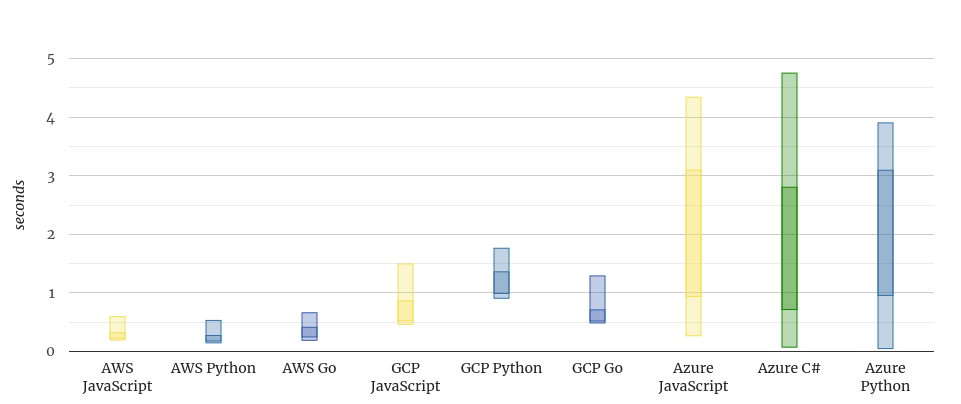
\includegraphics[width=\linewidth]{figs/ColdStart-programming-languages}
	\caption {اهمیت زبان و پلتفرم بدون سرور در تاخیر شروع سرد}
	\label{fig:ColdStart-programming-languages}
\end{figure}

\par
همانگونه که در تصویر \ref{fig:ColdStart-programming-languages} می‌بینیم، این آماده سازی شامل آماده سازی کانتینر‌ها، آماده سازی تابع، اختصاص منابع به کانتینر و در نهایت، اجرا در پلتفرم است. این تاخیر بسیار قابل توجه است و در شکل \ref{fig:coldstart-importance} نیز به خوبی نشان داده شده است. 

\par
همچنین،‌ یکی از مواردی که شروع سرد اتفاق می‌افتد، فراخوانی تابع برای اولین بار در پلتفرم است. 

حال چه عواملی در شروع سرد نقش دارند؟ عوامل عمده‌ای در این کار دخیل هستند ولی مهم‌ترین آن‌ها زبان برنامه‌نویسی و نوع پلتفرمی که در آن کد را اجرا می‌کنیم و کانفیگ نرم‌افزاری و سخت‌افزاری آن پلتفرم است. 

در مورد اهمیت زبان‌های برنامه نویسی می‌توان گفت چون زبان‌های مختلف زمان اجراهای متفاوتی دارند بنابراین موثر هستد. شکل زیر اهمیت زبان‌های برنامه‌نویسی را نشان می‌دهد. در این شکل از پلتفرم‌های مختلف برای اجرای توابع مختلف برای محاسبه‌ی زمان اجرا با درنظر گرفتن تاخیر شروع سرد استفاده شده است. 

در آزمایش دیگری با جاوا اسکریپت تابع‌های یکسانی نوشته شده با این تفاوت که حجم کتابخانه‌های هر تابع متفاوت است. این آزمایش در پلتفرم‌های مختلف نیز انجام شده و نتیجه طبق شکل زیر رسم شده است. 

\begin{figure}
	\centering
	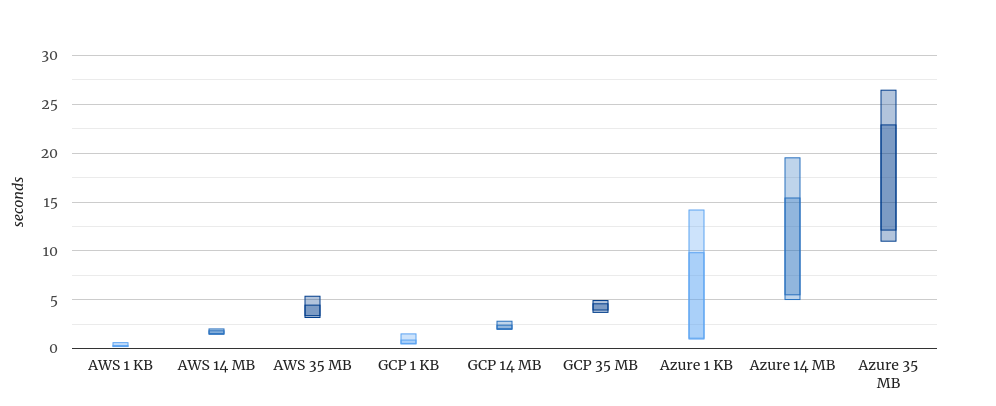
\includegraphics[width=\linewidth]{figs/ColdStart-programming-language-libraries}
	\caption {اهمیت اندازه کتابخانه برنامه  در تاخیر شروع سرد}
	\label{fig:ColdStart-programming-language-libraries}
\end{figure}

بنابراین با توجه به شکل \ref{fig:ColdStart-programming-language-libraries} می‌توان نتیجه گرفت حجم کتابخانه توابع نیز در مدت زمان تاخیر شروع سرد بسیار موثر است. 